%%This is a very basic article template.
%%There is just one section and two subsections.
\documentclass{article}

\usepackage{graphicx}

\begin{document}


\section{Introduction}

Model-based development environment for embedded systems. This document
describes the basic concepts used in embedded modeling.

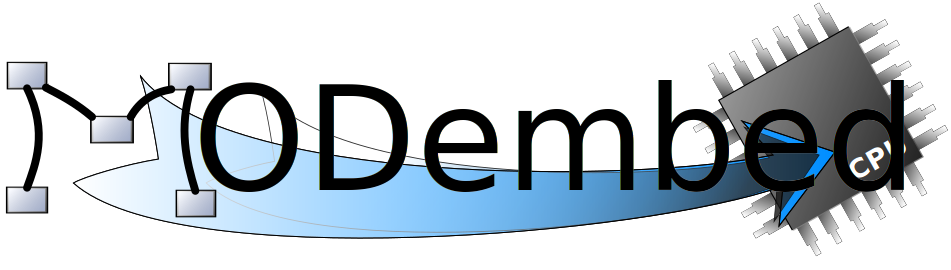
\includegraphics[width=115mm]{graphics/MODembed.pdf}

\subsection{Platform modeling}

This section describes the models used to define the high-level platform on
which the program models can be based on.

\subsubsection{Instruction set}

The most low-level model and the first thing is to be defined about an
architecture is the supported set of instructions. These instructions
are defined using a textual notation, and supports varying-length instructions
with fixed-length instruction words.



\subsubsection{Datatypes and Operations model}

\subsubsection{Platform definition}

\subsection{Program model}

More plain text.

\subsection{System model}

\end{document}
